\documentclass{standalone}
\usepackage{tikz}
\usetikzlibrary{patterns, positioning}

\begin{document}
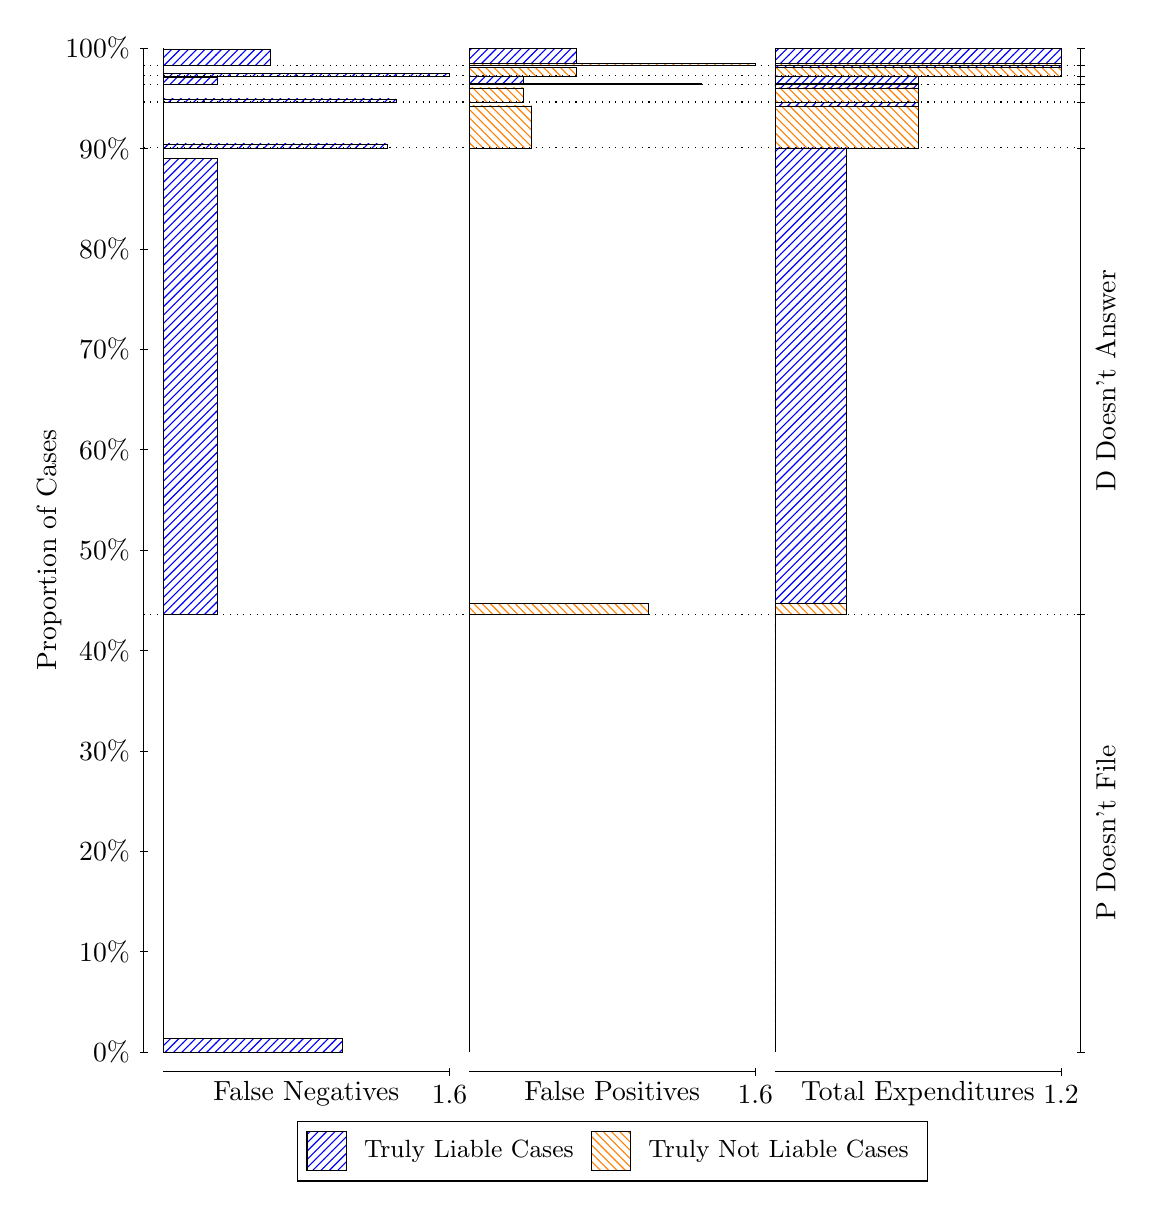
\begin{tikzpicture}
\draw[black, very thin] (1.5,1.75) -- (1.5,14.5);
\node[rotate=90, anchor=center] at (0.3, 8.125) {Proportion of Cases};
\draw[black, very thin] (1.45,1.75) -- (1.55,1.75);
\node[anchor=east] at (1.45, 1.75) {0\%};
\draw[black, very thin] (1.45,3.025) -- (1.55,3.025);
\node[anchor=east] at (1.45, 3.025) {10\%};
\draw[black, very thin] (1.45,4.3) -- (1.55,4.3);
\node[anchor=east] at (1.45, 4.3) {20\%};
\draw[black, very thin] (1.45,5.575) -- (1.55,5.575);
\node[anchor=east] at (1.45, 5.575) {30\%};
\draw[black, very thin] (1.45,6.85) -- (1.55,6.85);
\node[anchor=east] at (1.45, 6.85) {40\%};
\draw[black, very thin] (1.45,8.125) -- (1.55,8.125);
\node[anchor=east] at (1.45, 8.125) {50\%};
\draw[black, very thin] (1.45,9.4) -- (1.55,9.4);
\node[anchor=east] at (1.45, 9.4) {60\%};
\draw[black, very thin] (1.45,10.675) -- (1.55,10.675);
\node[anchor=east] at (1.45, 10.675) {70\%};
\draw[black, very thin] (1.45,11.95) -- (1.55,11.95);
\node[anchor=east] at (1.45, 11.95) {80\%};
\draw[black, very thin] (1.45,13.225) -- (1.55,13.225);
\node[anchor=east] at (1.45, 13.225) {90\%};
\draw[black, very thin] (1.45,14.5) -- (1.55,14.5);
\node[anchor=east] at (1.45, 14.5) {100\%};

\draw[black, very thin] (13.4,1.75) -- (13.4,14.5);
\draw[black, very thin] (13.35,1.75) -- (13.45,1.75);
\node[anchor=west] at (13.35, 1.75) {};
\draw[black, very thin] (13.35,7.3108) -- (13.45,7.3108);
\node[anchor=west] at (13.35, 7.3108) {};
\draw[black, very thin] (13.35,13.233) -- (13.45,13.233);
\node[anchor=west] at (13.35, 13.233) {};
\draw[black, very thin] (13.35,13.814) -- (13.45,13.814);
\node[anchor=west] at (13.35, 13.814) {};
\draw[black, very thin] (13.35,14.035) -- (13.45,14.035);
\node[anchor=west] at (13.35, 14.035) {};
\draw[black, very thin] (13.35,14.146) -- (13.45,14.146);
\node[anchor=west] at (13.35, 14.146) {};
\draw[black, very thin] (13.35,14.283) -- (13.45,14.283);
\node[anchor=west] at (13.35, 14.283) {};
\draw[black, very thin] (13.35,14.5) -- (13.45,14.5);
\node[anchor=west] at (13.35, 14.5) {};

\draw[black, very thin, pattern color=blue, pattern=north east lines] (1.75,1.75) rectangle (4.0208,1.9253);
\draw[black, very thin, pattern color=orange, pattern=north west lines] (1.75,1.9253) rectangle (1.75,7.3108);
\draw[black, very thin, pattern color=blue, pattern=north east lines] (1.75,7.3108) rectangle (2.4312,13.101);
\draw[black, very thin, pattern color=orange, pattern=north west lines] (1.75,13.101) rectangle (1.75,13.233);
\draw[black, very thin, pattern color=blue, pattern=north east lines] (1.75,13.233) rectangle (4.5885,13.282);
\draw[black, very thin, pattern color=orange, pattern=north west lines] (1.75,13.282) rectangle (1.75,13.814);
\draw[black, very thin, pattern color=blue, pattern=north east lines] (1.75,13.814) rectangle (4.7021,13.854);
\draw[black, very thin, pattern color=orange, pattern=north west lines] (1.75,13.854) rectangle (1.75,14.035);
\draw[black, very thin, pattern color=blue, pattern=north east lines] (1.75,14.035) rectangle (2.4312,14.129);
\draw[black, very thin, pattern color=orange, pattern=north west lines] (1.75,14.129) rectangle (1.75,14.146);
\draw[black, very thin, pattern color=blue, pattern=north east lines] (1.75,14.146) rectangle (5.3833,14.175);
\draw[black, very thin, pattern color=orange, pattern=north west lines] (1.75,14.175) rectangle (1.75,14.283);
\draw[black, very thin, pattern color=blue, pattern=north east lines] (1.75,14.283) rectangle (3.1125,14.479);
\draw[black, very thin, pattern color=orange, pattern=north west lines] (1.75,14.479) rectangle (1.75,14.5);
\draw[black, very thin, pattern color=orange, pattern=north west lines] (5.6333,1.75) rectangle (5.6333,7.1355);
\draw[black, very thin, pattern color=blue, pattern=north east lines] (5.6333,7.1355) rectangle (5.6333,7.3108);
\draw[black, very thin, pattern color=orange, pattern=north west lines] (5.6333,7.3108) rectangle (7.9042,7.4423);
\draw[black, very thin, pattern color=blue, pattern=north east lines] (5.6333,7.4423) rectangle (5.6333,13.233);
\draw[black, very thin, pattern color=orange, pattern=north west lines] (5.6333,13.233) rectangle (6.4281,13.765);
\draw[black, very thin, pattern color=blue, pattern=north east lines] (5.6333,13.765) rectangle (5.6333,13.814);
\draw[black, very thin, pattern color=orange, pattern=north west lines] (5.6333,13.814) rectangle (6.3146,13.994);
\draw[black, very thin, pattern color=blue, pattern=north east lines] (5.6333,13.994) rectangle (5.6333,14.035);
\draw[black, very thin, pattern color=orange, pattern=north west lines] (5.6333,14.035) rectangle (8.5854,14.052);
\draw[black, very thin, pattern color=blue, pattern=north east lines] (5.6333,14.052) rectangle (6.3146,14.146);
\draw[black, very thin, pattern color=orange, pattern=north west lines] (5.6333,14.146) rectangle (6.9958,14.253);
\draw[black, very thin, pattern color=blue, pattern=north east lines] (5.6333,14.253) rectangle (5.6333,14.283);
\draw[black, very thin, pattern color=orange, pattern=north west lines] (5.6333,14.283) rectangle (9.2667,14.304);
\draw[black, very thin, pattern color=blue, pattern=north east lines] (5.6333,14.304) rectangle (6.9958,14.5);
\draw[black, very thin, pattern color=orange, pattern=north west lines] (9.5167,1.75) rectangle (9.5167,7.1355);
\draw[black, very thin, pattern color=blue, pattern=north east lines] (9.5167,7.1355) rectangle (9.5167,7.3108);
\draw[black, very thin, pattern color=orange, pattern=north west lines] (9.5167,7.3108) rectangle (10.425,7.4423);
\draw[black, very thin, pattern color=blue, pattern=north east lines] (9.5167,7.4423) rectangle (10.425,13.233);
\draw[black, very thin, pattern color=orange, pattern=north west lines] (9.5167,13.233) rectangle (11.333,13.765);
\draw[black, very thin, pattern color=blue, pattern=north east lines] (9.5167,13.765) rectangle (11.333,13.814);
\draw[black, very thin, pattern color=orange, pattern=north west lines] (9.5167,13.814) rectangle (11.333,13.994);
\draw[black, very thin, pattern color=blue, pattern=north east lines] (9.5167,13.994) rectangle (11.333,14.035);
\draw[black, very thin, pattern color=orange, pattern=north west lines] (9.5167,14.035) rectangle (11.333,14.052);
\draw[black, very thin, pattern color=blue, pattern=north east lines] (9.5167,14.052) rectangle (11.333,14.146);
\draw[black, very thin, pattern color=orange, pattern=north west lines] (9.5167,14.146) rectangle (13.15,14.253);
\draw[black, very thin, pattern color=blue, pattern=north east lines] (9.5167,14.253) rectangle (13.15,14.283);
\draw[black, very thin, pattern color=orange, pattern=north west lines] (9.5167,14.283) rectangle (13.15,14.304);
\draw[black, very thin, pattern color=blue, pattern=north east lines] (9.5167,14.304) rectangle (13.15,14.5);
\draw[black, dotted] (1.5,7.3108) -- (13.4,7.3108);
\draw[black, dotted] (1.5,13.233) -- (13.4,13.233);
\draw[black, dotted] (1.5,13.814) -- (13.4,13.814);
\draw[black, dotted] (1.5,14.035) -- (13.4,14.035);
\draw[black, dotted] (1.5,14.146) -- (13.4,14.146);
\draw[black, dotted] (1.5,14.283) -- (13.4,14.283);
\draw[black, very thin] (1.75,1.5) -- (5.3833,1.5);
\node[anchor=north] at (3.5667, 1.5) {False Negatives};
\draw[black, very thin] (5.3833,1.45) -- (5.3833,1.55);
\node[anchor=north] at (5.3833, 1.45) {1.6};

\draw[black, very thin] (5.6333,1.5) -- (9.2667,1.5);
\node[anchor=north] at (7.45, 1.5) {False Positives};
\draw[black, very thin] (9.2667,1.45) -- (9.2667,1.55);
\node[anchor=north] at (9.2667, 1.45) {1.6};

\draw[black, very thin] (9.5167,1.5) -- (13.15,1.5);
\node[anchor=north] at (11.333, 1.5) {Total Expenditures};
\draw[black, very thin] (13.15,1.45) -- (13.15,1.55);
\node[anchor=north] at (13.15, 1.45) {1.2};

\node[black, centered, rotate=90] at (13.72, 4.5304) {P Doesn't File};
\node[black, centered, rotate=90] at (13.72, 10.272) {D Doesn't Answer};






\draw (7.449999999999999,1.5) node[draw=none] (baseCoordinate) {};
\begin{scope}[align=center]
        \matrix[scale=0.5, draw=black, below=0.5cm of baseCoordinate, nodes={draw}, column sep=0.1cm]{
            \node[rectangle, draw, minimum width=0.5cm, minimum height=0.5cm, pattern=north east lines, pattern color=blue] {}; &
            \node[draw=none, font=\small] (B) {Truly Liable Cases}; &
            \node[rectangle, draw, minimum width=0.5cm, minimum height=0.5cm, pattern=north west lines, pattern color=orange] {}; &
            \node[draw=none, font=\small] (B) {Truly Not Liable Cases}; \\
            };
\end{scope}

\end{tikzpicture}
\end{document}